\subsection{Alur Simulasi Perilaku Pengguna}

Gambar \ref{fig:user-flow} mengilustrasikan alur simulasi pengguna. Alur dimulai dengan pengguna virtual mengambil data acara, dilanjutkan dengan membaca data ketersediaan berdasarkan area dan kursi. Proses dilanjutkan dengan pemesanan, pembayaran (baik pembayaran berhasil atau gagal yang disimulasikan), dan verifikasi hasil pemesanan tiket.

\begin{figure}[H]
    \centering
    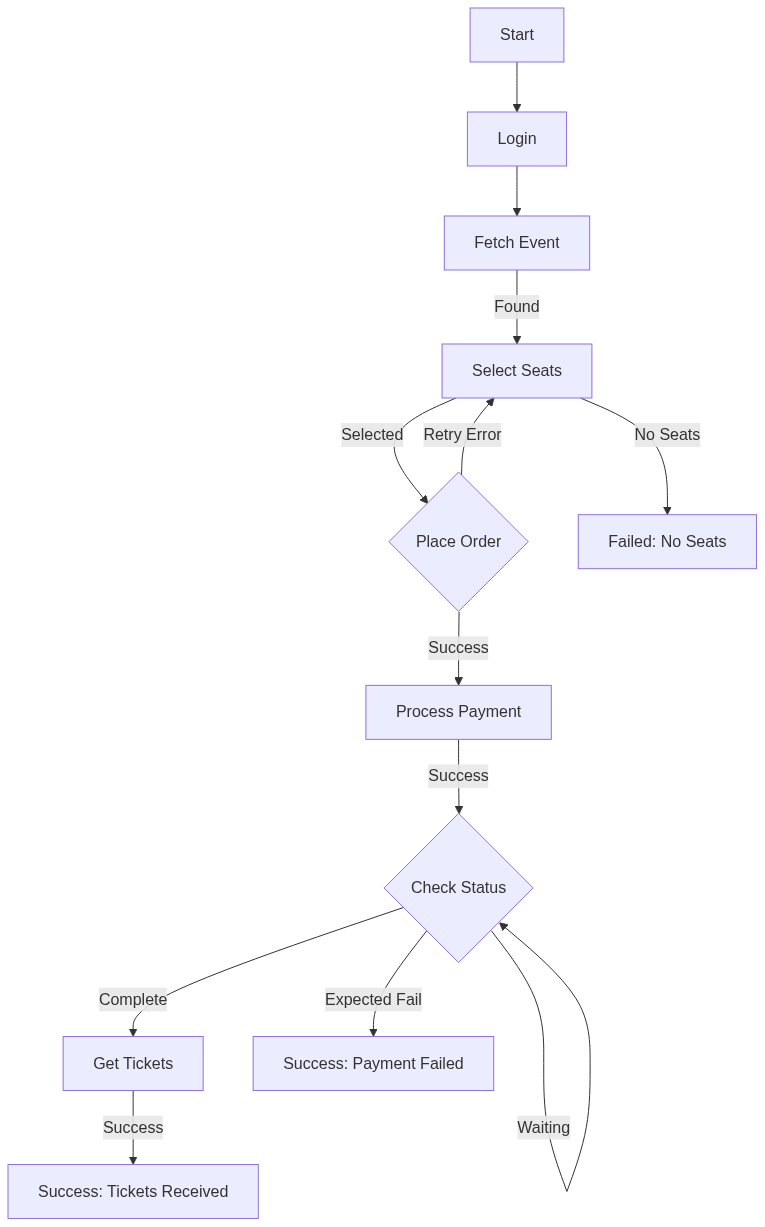
\includegraphics[width=0.7\textwidth]{resources/chapter-3/user-flow.png}
    \caption{Alur Simulasi Perilaku Pengguna}
    \label{fig:user-flow}
\end{figure}

\pagebreak